\documentclass[12pt]{report}

\usepackage[utf8]{inputenc}
\usepackage[francais]{babel}
\usepackage{graphicx}


\title{Rapport - Projet technologique - Hashiwokakero}
\author{Groupe TM2H}

\begin{document}

\maketitle

\begin{abstract}
Ceci est le résumé du rapport.
\end{abstract}

\tableofcontents

\chapter{Implantation de la librarie hashi}

\section{Création des fonctions de base}

\subsection{Les fonctions de node.c}
\textnormal{Après avoir compris le principe de base d'une partie hashiwokakero, il a était très facile de définir un \textbf{node} : il est composé de ses coordonnées et de son degré. Les fonctions de node.c sont relativement simples puisqu'elles sont simplement là pour créer, accéder à et supprimer la structure node définie de cette manière:}
\begin{verbatim}
typedef struct node_s {
	int x;
	int y;
	int required_degree;
} *node;
\end{verbatim}

\textnormal{Nous n'avons pas eu de difficulté a réaliser cette partie, surtout que le fichier qui nous était donné comme guide (node.h) contenait toutes les informations pour réaliser les fonctions. Le plus dur dans la création des fonctions de base se trouve dans le game.c}
\subsection{Les fonctions de game.c}
\textnormal{En effet, les fonctions composant game.c ont été un peu plus dur à réaliser. Tout d'abord, il a fallut définir la structure game qui contient les noeuds de la partie, le nombre de noeuds et les ponts.\\ Pour les noeuds, rien de bien compliqué : il suffit de créer un tableau de noeud et de donner à la structure le pointeur sur le premier élément. Pour les ponts, il a fallut un peu plus réfléchir, mais nous avons fini par créer une matrice de la taille du nombre de noeuds par le nombre de directions (c'est-à-dire 4). Voilà à quoi ressemble donc notre structure game :}
\begin{verbatim}
typedef struct game_s {
  int nb_nodes;
  node *nodes; 
  int **bridges;
} *game;
\end{verbatim}

\textnormal{Une fois la structure correctement définie, il a fallut réaliser les fonctions de création et de destruction d'une partie. Après quelques tests avec valgrind, tout semblait correct.\\ Nous nous sommes donc attaqués au gros du sujet : les fonctions qui font vivre ces structures game et node (l'ajout de pont, la supression de pont, le test de fin de partie...). Au fur et à mesure de notre avancement, les tests nous ont permis de déceller de nombreux bugs et nous éviter de nombreuses heures de débuggage même si gdb et valgrind nous ont énormément servi durant cette période.\\ Les fonctions les plus complexes qui nous ont demandé beaucoup de temps sont : can\_add\_bridge\_dir et game\_over.}

\subsubsection{La fonction can\_add\_bridge\_dir}
\textnormal{Cette fonction est l'une des plus utiles du jeu : elle permet de savoir s'il est possible ou non d'ajouter un pont. Il faut donc vérifier qu'il y ait un noeud dans la direction et que le pont ne croise pas un autre pont déjà existant. Pour la première vérification c'est assez simple puisque nous disposons déjà d'une fonction qui fait ça. Pour la deuxième vérification, après avoir cherché un bon moment, nous avons choisi de représenter nos ponts sous forme de vecteurs et de vérifier par le calcul vectoriel si notre pont croise un autre pont. \\ Supposons que le vecteur AB est notre pont et le vecteur CD l'autre pont, alors si vectoriel(vecteur(AB),vecteur(CD)) != 0, les deux vecteurs se croisent, mais il faut vérifier s'ils se croisent sur le segment CD avec vectoriel(vecteur(AB),vecteur(AD)) * vectoriel(vecteur(AB),vecteur(AC)) < 0\\On a donc une fonction qui prend de la place car il faut récupérer toutes les coordonnées des vecteurs, mais qui est plutôt simple.}

\subsubsection{La fonction game\_over}

\chapter{Interface terminal}
\textnormal{Lors de l'utilisation des game.o et node.o (puisque game.c et node.c n'étaient pas encore codés), nous avons dû utiliser quelque chose de suffisament visuel pour pouvoir détecter les éventuelles erreurs : une interface texte. Il a donc fallut créer une fonction qui prennait en paramètre la taille du jeu (size), un tableau double (grille[size][size]) où chaque case du jeu correspond à une valeur et le jeu lui même (jeu) définit par la structure game.
Voici l'affichage principal de la grille je jeu :}
\begin{verbatim}
for(int y = size-1; y >= 0; y--){
  for(int x = 0; x < size; x++){
    switch (grille[x][y]){
      case -1: printf(" .  "); break;
      case -2: printf(" +  "); break;
      case -3: printf(" #  "); break;
      default: printf(" %d  ", grille[x][y]); break;
    }
  }
}
\end{verbatim}
On peut voir que grille[x][y] peut avoir pour valeur :
\begin{itemize}
\item -1 : cas où l'on affiche un espace sans pont (.)
\item -2 : cas où l'on affiche un pont simple (+)
\item -3 : cas où l'on affiche un pont double (\#)
\item ? : toute autre valeur correspond au degré d'un noeud, on l'affiche
\end{itemize}
Nous avons donc regardé la partie et corrigé les problèmes avec ces lignes, l'affichage permettant alors de connaître toute la composition du jeu.

\chapter{Caprice des profs}

\chapter{Solveur}
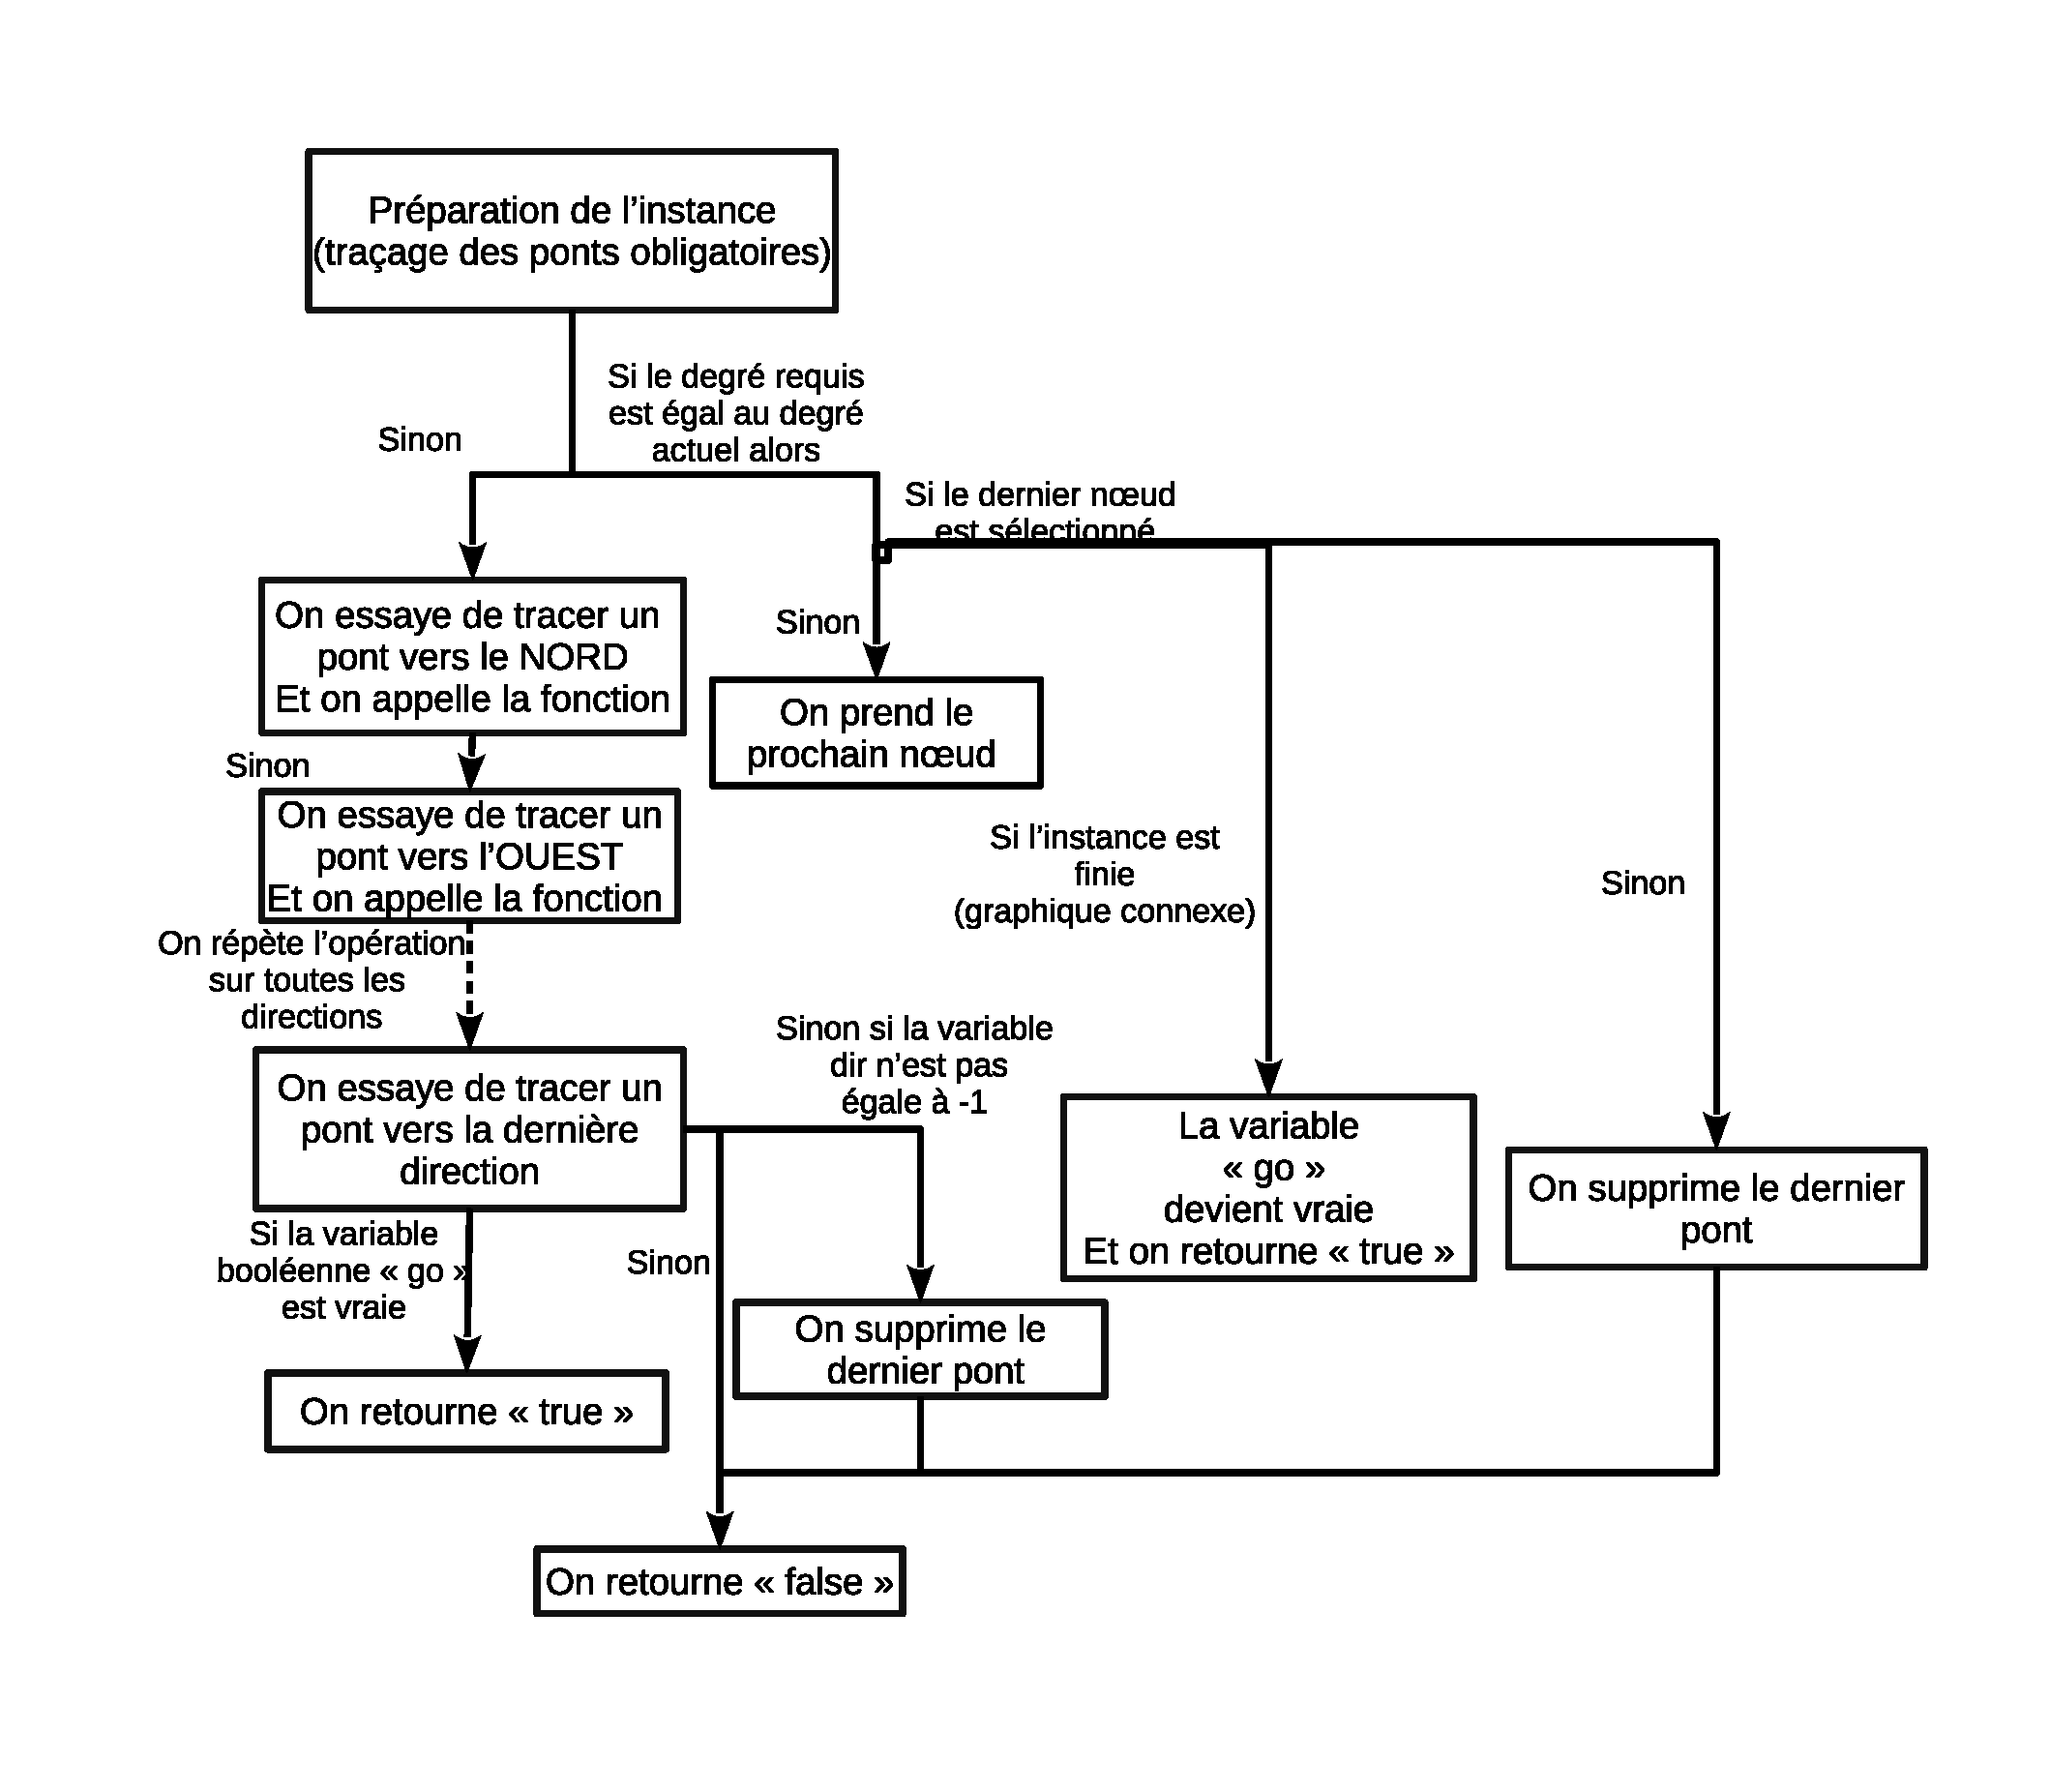
\includegraphics[width = 1.00\textwidth]{explication_solveur.eps}
\section{Explication du graphique}
La préparation de l'instance consiste à tracer les ``ponts obligatoires'', ceci concerne les îles qui n'ont qu'une possibilité de lien(s),
on a déterminé plusieurs cas:\newline
- Deux îles ne peuvent pas se compléter totalement mutuellement, ce qui formerait un bloc connexe.\newline
- Si une île a un nombre de ponts possibles maximum (en fonction des voisins possiblement atteignables) égal à son degré requis, on doit tracer tous ses ponts.\newline

Les arguments de la fonction sont:
\begin{itemize}
\item l'instance de jeu (g)
\item le numéro de l'île où nous allons appliquer nos opérations (node\_num)
\item la direction du dernier pont posé utile quand on dépile pour retirer le dernier pont (dir)
\item une variable indiquant si la solution a été trouvée (go)
\end{itemize}

\section{Possibilité d'amélioration}
Pour améliorer ce solveur on pourrait refaire le processus de ``ponts obligatoire'' à chaque fois que l'on fait une action, mais celà implique d'avoir une sauvegarde de l'état du jeu pour que lorsque l'on dépile on puisse retirer les ponts posés par ce processus. On pourrait aussi améliorer 

\newpage
\chapter{Interface graphique}
\newpage
\chapter{Bonus: Portabilité sur Android}
\newpage
\end{document}

